%
% Configuración y uso de Git
%

\chapter[Uso de Git y diferencias con Subversion]{
	Uso de sistema de control de versiones Git
	\label{ap:git}
}

Los dos sistemas de control de versiones más comunes en el mercado del desarrollo de software son SVN y Git. La principal diferencia entre ambos es que uno gestiona los cambios de manera centralizada, y por el otro lado, se realiza de forma distribuida. Sin embargo, a continuación se detallarán las distinciones más importantes.

%
% Sección diferencias entre Git y SVN
%
\section{Diferencias entre Git y SVN \label{sec:git_vs_svn}}

La lista detallada con una comparación exhaustiva sobre Git y SVN puede encontrarse en \cite{svnvsgit}. Debido a que es un documento muy extenso, se hará alusión a las diferencias destacadas.

\begin{itemize}
	\item{
		Git es mucho más rápido que Subversion.
	}	
	\item{
		Subversion permite permite realizar «checkout» sólo a un subárbol del repositorio; Git requiere que se clone el repositorio entero (incluyendo la historia) y crear una copia de trabajo a partir de uno de los árboles.
	}
	\item{
		Los repositorios de Git son mucho más pequeños que los de SVN (para el proyecto Mozilla, aprox. 30 veces más pequeño).
	}
	\item{
		Git fue diseñado para ser totalmente distribuido desde el inicio, permitiendo a cada desarrollador tener un control total en una versión local.
	}
	\item{
		Las ramas en Git son más simples y requieren menos recursos que en SVN.
	}
	\item{
		Las ramas en Git incluyen toda su historia.
	}
	\item{
		Git provee de mecanismos para una mejor auditoría de ramas y eventos de fusión de ramas.
	}
	\item{
		Los formatos de fichero de los repositorios Git son simples, por lo que repararlos es fácil y muy eventualmente se producirán casos de corrupción.
	}
	\item{
		SVN es centralizado y Git descentralizado, por lo que hacer copias de seguridad en SVN es muxo más sencillo. En Git habría que seleccionar la carpeta o rama que se quiere respaldar.
	}
	\item{
		Clonar un repositorio en Git implica copiar el repositorio entero.
	}
	\item{
		La interfaz de usuario de SVN está más madura que la de Git.
	}
	\item{
		Recorrer las versiones es más simple en SVN debido a que se usan números de revisión secuencial; Git usa descriptores hash impredecibles. En Git, ir hacia atrás sobre el repositorio es fácil usando la sintaxis ``\textasciicircum'', pero no hay manera fácil de ir hacia delante.
	}
\end{itemize}

%
%	Sección Uso de Git Uso de Git
%
\section{Uso de Git}
Para poder manejar un sistema de control de versiones, se puede crear un servidor exclusivo para ello o utilizar algún servicio que permita almacenar repositorios.

%
%	Subseccion Darse de alta en servicio GitHub
%
\subsection{Darse de alta en servicio GitHub}

Un ejemplo del segundo caso es usar {\it GitHub} (\url{http://www.github.com}), el cuál es un servicio --- desarrollado utilizando el {\it framework Ruby on Rails} --- donde, de forma gratuita, se pueden alojar proyectos. 

Por tanto, una vez en el portal del servicio, se crea una cuenta y se añaden repositorios para cada una de las aplicaciones en las que se esté trabajando.

Una de las ventajas de usar este servicio es que no se necesita poner recursos propios de la empresa para mantener el control de versiones. Además, el nivel de configuración es bastante alto, permitiendo que se puedan hacer repositorios públicos o privados; dar permisos para trabajar en equipo sobre un mismo proyecto; crear wikis o enlazar el gestor de versiones con otros servicios que se usen en el proyecto (Basecamp, PivotalTracker, Twitter, etc.).

%
%	Subseccion Instalar Git en el equipo de trabajo
%
\subsection{Instalar Git en el equipo de trabajo \label{sub:inst_git}}

Desde \url{Github.com} se muestra una guía de instalación del software \cite{guia_inst_git}. Es multiplataforma, por lo se puede realizar tanto para entornos Linux, OSX o Windows.

%
%	Subseccion Gernerar llaves SSH
%
\subsection{Generar llaves SSH}

La generación de llaves SSH necesarias para el funcionamiento correcto del servicio, se detalla en el enlace que aparece en \ref{sub:inst_git}.

El procedimiento básico es el de, primeramente, generar un par de llaves RSA. A continuación se añadiría la llave a la cuenta de Github.

\begin{center}{
	\fboxsep 10px
	\fcolorbox{white}{gray}{\parbox{0.95\textwidth}{
		{\bf \$} ssh-keygen -t rsa -C ``direccion@correo.com''
	}}}
\end{center}

\begin{center}{
	\fboxsep 10px
	\fcolorbox{white}{gray}{\parbox{0.95\textwidth}{
		{\bf \$} cat \textasciitilde /.ssh/id\mathunderscore rsa.pub \textbar pbcopy
	}}
}
\end{center}

Con el comando pbcopy se copia la clave al portapapeles, la cuál hay que escribir en la sección de ``Añadir otra llave pública'' en ``{\it SSH Public Keys}''.

%
%	Subseccion Obteniendo un repositorio Git
%
\subsection{Obteniendo un repositorio Git}

Se puede obtener un proyecto Git de dos formas. La primera toma un proyecto o directorio existente y lo importa en Git. La segunda clona un repositorio Git existente de otro servidor.

Si se está empezando el seguimiento en Git de un proyecto existente, hay que ir al directorio del proyecto y escribir:

\begin{center}{
	\fboxsep 10px
	\fcolorbox{white}{gray}{\parbox{0.95\textwidth}{
		{\bf \$} git init
	}}}
\end{center}

Esto crea un nuevo subdirectorio llamado .git que contiene todos los archivos necesarios del repositorio --- un esqueleto de un repositorio Git.

Si se desea empezar a controlar versiones de archivos existentes (a diferencia de un directorio vacío), probablemente habría que comenzar el seguimiento de esos archivos y hacer una confirmación inicial. Esto se consigue con unos pocos comandos: {\it git add} para especificar qué archivos se quieren controlar, seguidos de un {\it commit} para confirmar los cambios:

\begin{center}{
	\fboxsep 10px
	\fcolorbox{white}{gray}{\parbox{0.95\textwidth}{
		{\bf \$} git add *.c\\
		{\bf \$} git add README\\
		{\bf \$} git commit -m ``versión inicial del proyecto''
	}}}
\end{center}

En este momento, se tendría un repositorio Git con archivos bajo seguimiento, y una confirmación inicial.

\subsubsection{Clonando un repositorio existente}

Si se desea obtener una copia de un repositorio Git existente --- por ejemplo, un proyecto en el que te gustaría contribuir --- el comando que se necesita es {\it git clone}. Con ello, cada versión de cada archivo de la historia del proyecto es descargado cuando se ejecuta el comando. De hecho, si el disco de tu servidor se corrompe, se puede usar cualquiera de los clones en cualquiera de los clientes para devolver al servidor al estado en el que estaba cuando fue clonado.

\begin{center}{
	\fboxsep 10px
	\fcolorbox{white}{gray}{\parbox{0.95\textwidth}{
		{\bf \$} git clone git://github.com/schacon/grit.git
	}}}
\end{center}

%
%	Subseccion Guardando cambios en el repositorio
%
\subsection{Guardando cambios en el repositorio}

Se tiene un repositorio Git completo, y una copia de trabajo de los archivos de ese proyecto. Es necesario hacer algunos cambios, y confirmar instantáneas de esos cambios al repositorio cada vez que el proyecto alcance un estado que desees grabar.

Cada archivo del directorio de trabajo puede estar en uno de estos dos estados: bajo seguimiento ({\it tracked}), o sin seguimiento ({\it untracked}). Los archivos bajo seguimiento son aquellos que existían en la última instantánea; pueden estar sin modificaciones, modificados, o preparados. Los archivos sin seguimiento son todos los demás --- cualquier archivo del directorio que no estuviese en la última instantánea ni está en el área de preparación. La primera vez que se clona un repositorio, todos los archivos estarán bajo seguimiento y sin modificaciones, ya que se acaban de copiar y no han sido modificados.

A medida que se editan archivos, Git los ve como modificados, porque se han cambiado desde la última confirmación. Se preparan estos archivos modificados y luego son confirmados los cambios que se hayan preparado, formando un ciclo que se repite. Este proceso queda ilustrado en la figura \ref{fig:ciclo_vida_estado_archivos}.

\begin{figure}
  \centering
    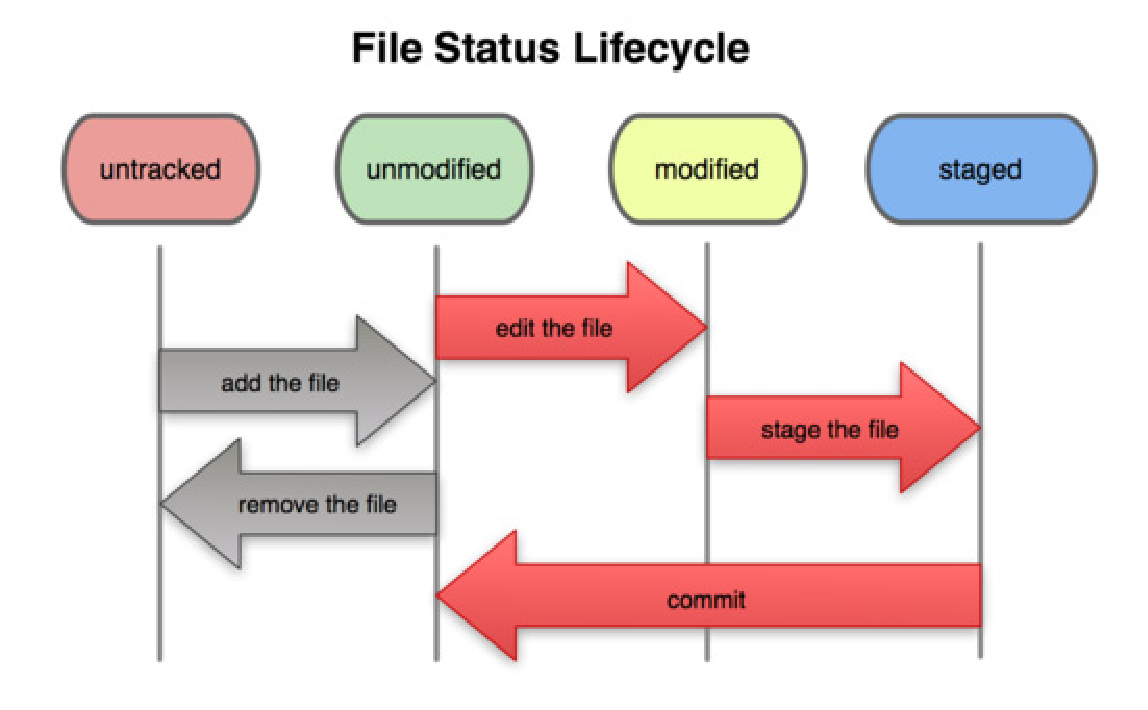
\includegraphics[width=350px]{./eps/git/git_ciclo_vida_status_archivos.eps}
  \caption{El ciclo de vida del estado de los archivos}
  \label{fig:ciclo_vida_estado_archivos}
\end{figure}

\subsubsection{Comprobando el estado de los archivos}

La principal herramienta para determinar qué archivos están en qué estado es el comando {\it git status}. Si se ejecuta este comando justo después de clonar un repositorio, se debería ver algo así:

\begin{center}{
	\fboxsep 10px
	\fcolorbox{white}{gray}{\parbox{0.95\textwidth}{
		{\bf \$} git status\\
		\# On branch master\\
		nothing to commit (working directory clean)
	}}}
\end{center}

\subsubsection{Seguimiento de nuevos archivos}

Para empezar el seguimiento de un nuevo archivo se usa el comando {\it git add}. El seguimiento del archivo README comienza ejecutando esto:

\begin{center}{
	\fboxsep 10px
	\fcolorbox{white}{gray}{\parbox{0.95\textwidth}{
		{\bf \$} git add README
	}}}
\end{center}

Si se vuelve a ejecutar el comando {\it git status}, se observa que {\it README} está ahora bajo seguimiento y preparado:

\begin{center}{
	\fboxsep 10px
	\fcolorbox{white}{gray}{\parbox{0.95\textwidth}{
		{\bf \$} git status\\
		\# On branch master\\
		\# Changes to be committed:\\
		\#   (use ``git reset HEAD file..'' to unstage)\\
		\#\\
		\#	new file:   README\\
		\#\\
	}}}
\end{center}

\subsubsection{Viendo los cambios preparados y no preparados}

El comando {\it git status} puede ser demasiado impreciso --- se quieren saber exactamente los cambios realizados, no sólo qué archivos fueron modificados. Por ello, se puede usar el comando {\it git diff}. Con el uso de {\it git diff} se muestran exactamente las líneas añadidas y eliminadas.

\begin{center}{
	\fboxsep 10px
	\fcolorbox{white}{gray}{\parbox{0.95\textwidth}{
		{\bf \$} git diff
	}}}
\end{center}

\subsubsection{Confirmando los cambios}

Ahora que el área de preparación está como se quiere, se pueden confirmar los cambios. Hay que recordar que cualquier cosa que todavía esté sin preparar ---cualquier archivo creado o modificado, y sobre el que no se haya ejecutado {\it git add} desde su última edición--- no se incluirá en esta confirmación. Se mantendrán como modificados en el disco.

En este caso, la última vez que se ejecutó {\it git status}, se comprobó que estaba todo preparado, por lo que se está listo para confirmar los cambios. La forma más fácil de confirmar es escribiendo {\it git commit}:

\begin{center}{
	\fboxsep 10px
	\fcolorbox{white}{gray}{\parbox{0.95\textwidth}{
		{\bf \$} git commit
	}}}
\end{center}

El editor mostrará el siguiente texto:

\begin{center}{
	\fboxsep 10px
	\fcolorbox{white}{gray}{\parbox{0.95\textwidth}{
		\# Please enter the commit message for your changes. Lines starting\\
		\# with ``\#'' will be ignored, and an empty message aborts the commit.\\
		\# On branch master\\
		\# Changes to be committed:\\
		\#   (use ``git reset HEAD file..'' to unstage)\\
		\#\\
		\#       new file:   README\\
		\#       modified:   benchmarks.rb\\
	}}}
\end{center}

%
% Subsection Trabajando con repositorios remotos
%
\subsection{Trabajando con repositorios remotos}

Para poder realizar la colaboración en un proyecto Git, se necesita saber cómo gestionar los repositorios remotos. Los repositorios remotos son versiones del proyecto que se encuentran alojados en Internet o en algún punto de la red. Puedes tener varios, cada uno de los cuales puede ser de sólo lectura, o de lectura/escritura, según los permisos que tengas. Colaborar con otros implica gestionar estos repositorios remotos, y mandar (push) y recibir (pull) datos de ellos cuando se necesite compartir información.

\subsubsection{Mostrando repositorios remotos}
Para ver qué repositorios remotos se tienen configurados, se ejecuta el comando {\it git remote}. Con él se muestra una lista con los nombres de los remotos que se hayan especificado. Cuando se clona un proyecto, por defecto Git le da el nombre de {\it origin}.

\begin{center}{
	\fboxsep 10px
	\fcolorbox{white}{gray}{\parbox{0.95\textwidth}{
		{\bf \$} git clone git://github.com/schacon/ticgit.git\\
		Initialized empty Git repository in /private/tmp/ticgit/.git/\\
		remote: Counting objects: 595, done.\\
		remote: Compressing objects: 100\\
		remote: Total 595 (delta 255), reused 589 (delta 253)\\
		Receiving objects: 100\\
		Resolving deltas: 100\\
		\$ cd ticgit\\
		\$ git remote\\
		origin
	}}}
\end{center}

\subsubsection{Añadiendo repositorios remotos}

Para añadir un nuevo repositorio Git remoto, asignándole un nombre con el que referenciarlo fácilmente, se ejecuta {\it git remote add [nombre] [url]}.

\begin{center}{
	\fboxsep 10px
	\fcolorbox{white}{gray}{\parbox{0.95\textwidth}{
		{\bf \$} git remote\\
		origin\\
		{\bf \$} git remote add pb git://github.com/paulboone/ticgit.git\\
		{\bf \$} git remote -v\\
		origin	git://github.com/schacon/ticgit.git\\
		pb	git://github.com/paulboone/ticgit.git\\
	}}}
\end{center}

\subsubsection{Recibiendo de los repositorios remotos}

Una vez añadido un nuevo repositorio, y siguiendo con el ejemplo anterior, se podría recuperar toda la información que no se tuviese en el repositorio local ejecutando {\it git fetch [remote-name]}.

\begin{center}{
	\fboxsep 10px
	\fcolorbox{white}{gray}{\parbox{0.95\textwidth}{
		{\bf \$} git fetch pb\\
		remote: Countin objects: 58, done.\\
		remote: Compressing objects: 100.\\
		remote: Total 44 (delta 24), reused 1 (delta 0)\\
		Unpacking objects: 100.\\
		From git://github.com/paulboone/ticgit\\
		new branch      master pb/master\\
		new branch      ticgit pb/ticgit\\
	}}}
\end{center}

Si se clona un repositorio, el comando añade automáticamente ese repositorio remoto con el nombre de ``origin''. Por tanto, {\it git fetch origin} recupera toda la información enviada a ese servidor desde que se clonó (o desde la última vez que se ejecutó el comando {\it fetch}). Es importante tener en cuenta que el comando {\it fetch} sólo recupera la información y la pone en el repositorio local ---no la une automáticamente con el trabajo ni modifica aquello en lo que se está trabajando. Hay que unir ambos manualmente a posteriori---.

Normalmente, si se ha configurado una rama para seguir otra rama remota, se puedes usar el comando {\it git pull} para recuperar y unir automáticamente la rama remota con la rama actual.

\subsubsection{Enviando a los respositorios remotos}

Cuando un proyecto se encuentra en un estado en el que se quiere compartir información, hay que enviarlo a un repositorio remoto. El comando que permite hacer esto es: {\it git push [nombre-remoto][nombre-rama]}. Si se quiere enviar la rama maestra (master) al servidor origen (origin), se ejecutaría la siguiente instrucción para enviar el trabajo al servidor:

\begin{center}{
	\fboxsep 10px
	\fcolorbox{white}{gray}{\parbox{0.95\textwidth}{
		{\bf \$} git push origin master
	}}}
\end{center}

Este comando funciona únicamente si se ha clonado de un servidor en el que se tiene permiso de escritura, y nadie ha enviado información mientras tanto. Si dos personas clonan a la vez, enviando uno su información y luego enviando el otro la suya, el segundo envío será rechazado. Se tendrá que bajar primero su trabajo e incorporarlo en su rama local para que se le permita hacer un envío.

\subsubsection{Eliminando repositorios remotos}

Si por algún motivo se quiere eliminar una referencia ---se ha movido el servidor o ya no se está usando un determinado {\it mirror}---se puede usar el comando {\it git remote rm}.

\begin{center}{
	\fboxsep 10px
	\fcolorbox{white}{gray}{\parbox{0.95\textwidth}{
		{\bf \$} git remote rm pb\\
		{\bf \$} git remote\\
		origin		
	}}}
\end{center}

%
% Subsection Ramificaciones en Git
%
\subsection{Ramificaciones en Git}

La verdadera potencia de un sistema de control de versiones radica en el uso de ramificaciones. Las buenas prácticas aconsejan que se creen nuevas ramificaciones donde se desarrollen nuevas funcionalidades y, posteriormente, se unan con la rama perteneciente a una versión estable. 

\subsubsection{¿Qué es una rama? \label{que_es_rama}}

Para entender realmente cómo ramifica Git, previamente hemos de examinar la forma en que almacena sus datos. Git no los almacena de forma incremental (guardando solo diferencias), sino que los almacena como una serie de instantáneas (copias puntuales de los archivos completos, tal y como se encuentran en ese momento).

En cada confirmación de cambios ({\it git commit}), Git realiza sumas de control de cada subcarpeta, y guarda en el repositorio Git una copia de cada uno de los archivos contenidos en ellas. Después, Git crea un objeto de confirmación con los metadatos pertinentes y un apuntador al nodo correspondiente del árbol de proyecto. Esto permitirá poder regenerar posteriormente dicha instantánea cuando sea necesario. 

Para ilustrarlo con un ejemplo, en un momento dado, el repositorio de Git contendrá cinco objetos: un ``blob'' para cada uno de los tres archivos, un árbol con la lista de contenidos de la carpeta (más sus respectivas relaciones con los ``blobs''), y una confirmación de cambios ({\it commit}) apuntando a la raíz de ese árbol y conteniendo el resto de metadatos pertinentes. Conceptualmente, el contenido del repositorio Git será algo parecido a la figura \ref{fig:ramas_conf_senc}.

\begin{figure}
  \centering
    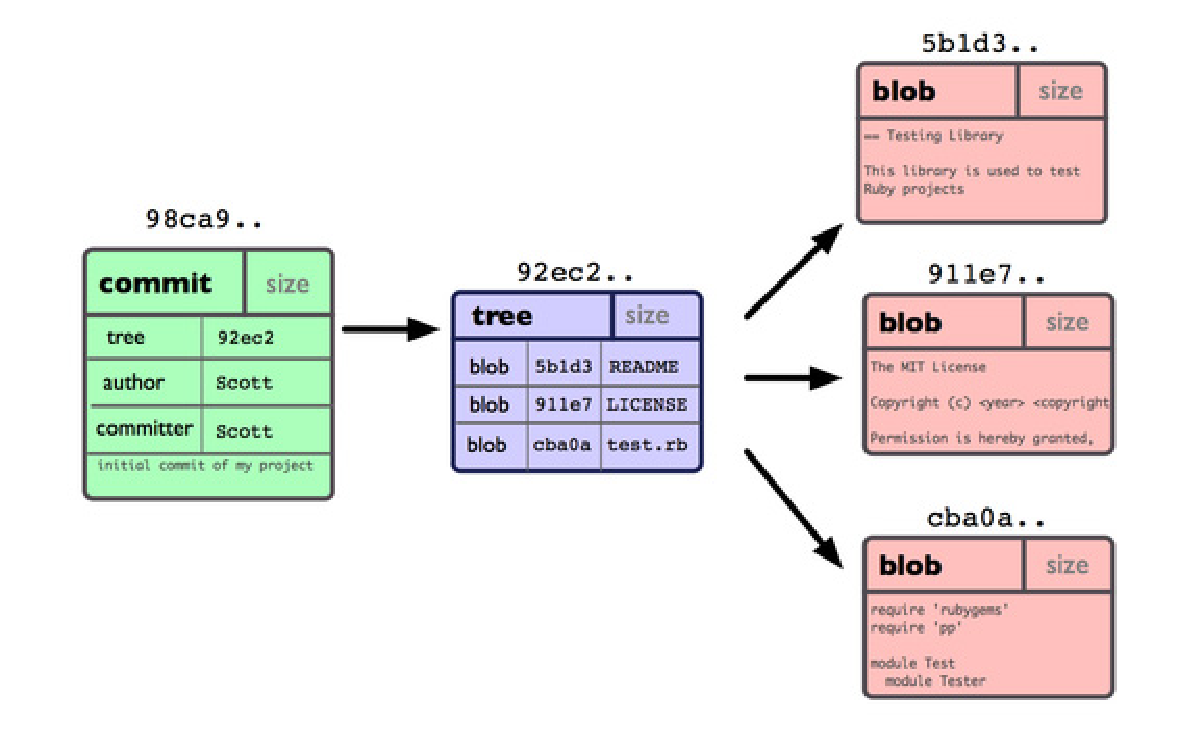
\includegraphics[width=350px]{./eps/git/git_datos_repositorio_confirmacion_sencilla.eps}
  \caption{Datos en el repositorio tras una confirmación sencilla}
  \label{fig:ramas_conf_senc}
\end{figure}

Si se hacen más de un cambio y se vuelven a confirmar, la siguiente confirmación guardará un apuntador a su confirmación precedente. Tras un par de confirmaciones más, el registro ha de ser algo parecido a la figura \ref{fig:ramas_conf_serie}.

\begin{figure}
  \centering
    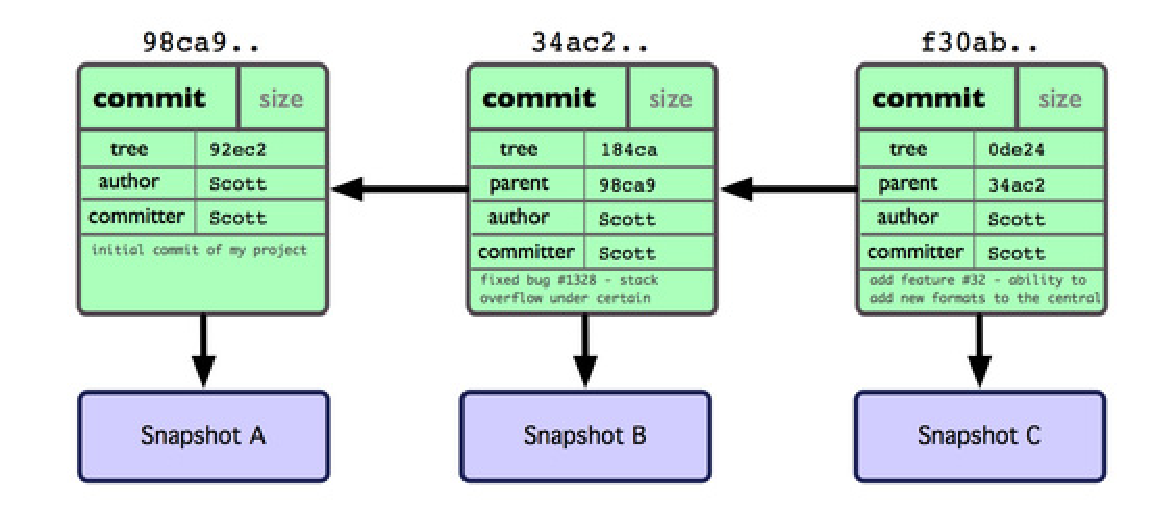
\includegraphics[width=350px]{./eps/git/git_datos_repositorio_serie_conf.eps}
  \caption{Datos en el repositorio tras una serie de confirmaciones}
  \label{fig:ramas_conf_serie}
\end{figure}

Una rama Git es simplemente un apuntador móvil apuntando a una de esas confirmaciones. La rama por defecto de Git es la rama ``master''. Con la primera confirmación de cambios que se realice, se creará esta rama principal ``master'' apuntando a dicha confirmación. En cada confirmación de cambios que se realice, la rama irá avanzando automáticamente. La rama ``master'' apuntará siempre a la última confirmación realizada (figura \ref{fig:ramas_apuntadores_reg}).

\begin{figure}
  \centering
    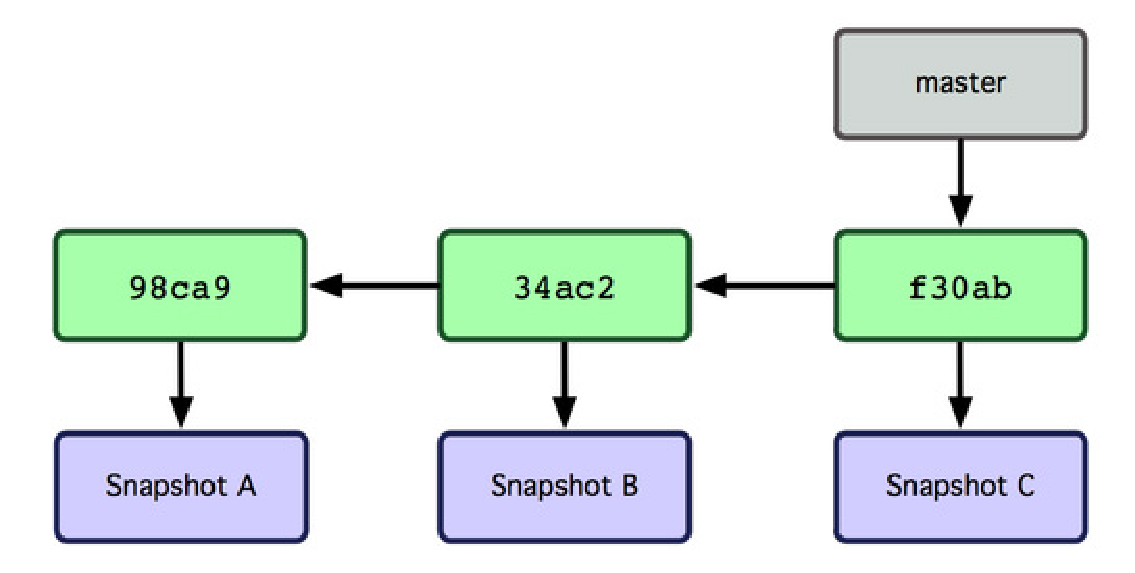
\includegraphics[width=350px]{./eps/git/git_apuntador_registro_conf_rama.eps}
  \caption{Apuntadores en el registro de confirmaciones de una rama}
  \label{fig:ramas_apuntadores_reg}
\end{figure}

Cuando se crea una nueva rama, simplemente se crea un nuevo apuntador para que se pueda mover libremente. Por ejemplo, si se quiere crear una nueva rama denominada ``testing'', se usará el comando {\it git branch}.

\begin{center}{
	\fboxsep 10px
	\fcolorbox{white}{gray}{\parbox{0.95\textwidth}{
		{\bf \$} git branch testing		
	}}}
\end{center}

Esto creará un nuevo apuntador apuntando a la misma confirmación donde se esté actualmente (figura \ref{fig:ramas_apuntadores_varias}).

\begin{figure}
  \centering
    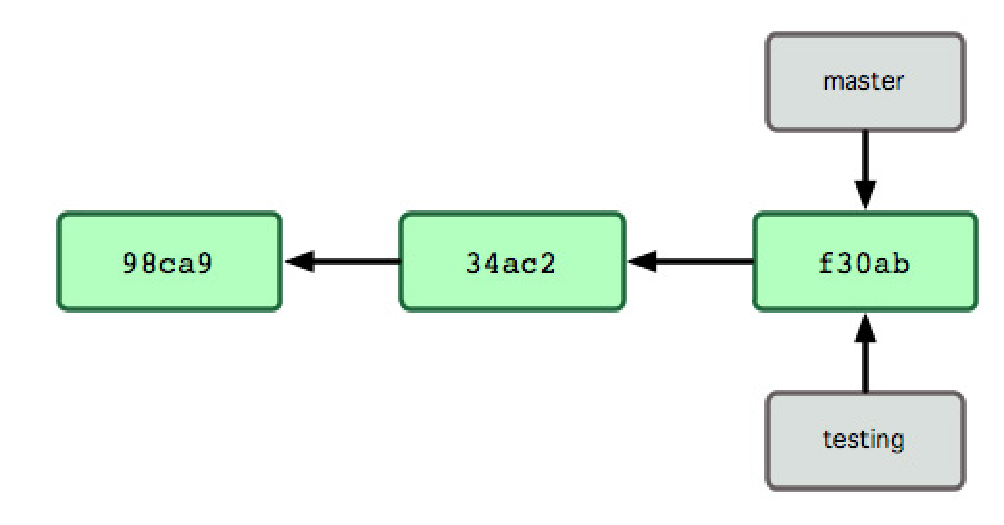
\includegraphics[width=350px]{./eps/git/git_apuntador_varias_ramas.eps}
  \caption{Apuntadores de varias ramas en el registro de confirmaciones de cambio}
  \label{fig:ramas_apuntadores_varias}
\end{figure}

Y, ¿cómo sabe Git en qué rama está en un momento determinado? Mediante un apuntador especial denominado HEAD (figura \ref{fig:ramas_apuntadores_head}). Aunque es preciso comentar que este HEAD es totalmente distinto al concepto de HEAD en otros sistemas de control de cambios como Subversion o CVS. En Git, es simplemente el apuntador a la rama local en la que se esté en ese momento. En este caso, en la rama ``master''. Puesto que el comando {\it git branch} solamente crea una nueva rama, y no salta a dicha rama.

\begin{figure}
  \centering
    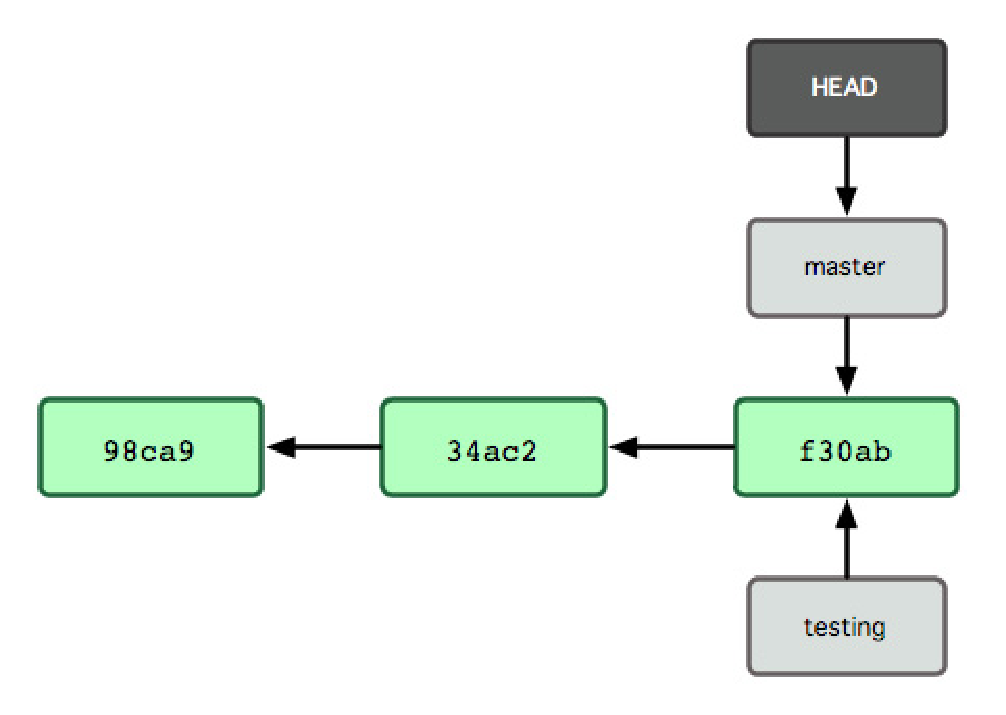
\includegraphics[width=350px]{./eps/git/git_apuntador_head.eps}
  \caption{Apuntador HEAD a la rama donde se esté actualmente}
  \label{fig:ramas_apuntadores_head}
\end{figure}

\subsubsection{Procedimientos básicos para ramificar y fusionar}

Como se menciona en la sección \ref{que_es_rama}, la potencia de Git radica en que se pueden usar ramas locales que posteriormente se pueden fusionar con ramas remotas. Con ello se consigue descentralizar el proceso de control de versiones.

Se va a presentar un ejemplo simple de ramificar y de fusionar, con un flujo de trabajo que se podría presentar en la realidad. Imagine los siguientes pasos:

\begin{enumerate}
	\item{Trabaja en la elabora.ción de un sitio web}
	\item{Crea una nueva rama para desarrollar el rediseño de un módulo.}
	\item{Sube la rama al repositorio remoto para que otros puedan trabajar sobre ella.}
	\item{Termina con el rediseño.}
	\item{Unifica con la versión estable.}
	\item{Elimina la rama creada para el rediseño en el repositorio remoto.}
\end{enumerate}

Una vez hecha la conexión al servidor con el repositorio remoto, lo que corresponde es crear una nueva rama para desarrollar el rediseño del módulo en cuestión. Con el comando {\it git branch [nombre-rama]} se puede crear una nueva rama, pero sin cambiar el puntero a ella. Por ello, con el uso del comando {\it git checkout -b [nombre-rama]} sí que se crea una nueva rama y se cambia el puntero a ella para trabajar sobre la misma.

\begin{center}{
	\fboxsep 10px
	\fcolorbox{white}{gray}{\parbox{0.95\textwidth}{
		{\bf \$} git checkout -b redesign\\
		M public/index.html\\
		Switched to a new branch ``redesign'' 
	}}}
\end{center}

Con este proceso se ha creado una nueva rama en el repositorio local. Lo ideal ahora es crear esta rama en el repositorio remoto, para que el resto del equipo pueda tirar de los cambios realizados en ella. 

\begin{center}{
	\fboxsep 10px
	\fcolorbox{white}{gray}{\parbox{0.95\textwidth}{
		{\bf \$} git push origin redesign
	}}}
\end{center}

Hay que recordar que si quiere conocer la rama en la que está situado el puntero, el comando {\it git branch} sin parámetros lo especifica.

Volviendo a la situación de partida, se está en el punto en que ya se ha creado una rama para el rediseño y se ha subido al repositorio remoto para que otros puedan trabajar sobre ella. Ahora, para obtener la versión estable sobre la cuál trabajar, habría que descargarse el contenido de la rama ``master''.

\begin{center}{
	\fboxsep 10px
	\fcolorbox{white}{gray}{\parbox{0.95\textwidth}{
		{\bf \$} git pull origin\\
		{\bf \$} git merge master
	}}}
\end{center}

Esta combinación de comandos le dice a Git que tire todos los cambios desde el repositorio origin, incluyendo todas las ramas. Entonces, se combinará la rama ``master'' con ``redesign'', sobre la que se desarrollarán los cambios.

Al finalizar con el desarrollo del rediseño del módulo ---haciendo las pruebas de verificación--- hay que realizar el proceso contrario: combinar la rama ``redesign'' con ``master'' para conseguir una versión estable. Primero se cambia a la rama ``master'' y luego se realiza la fusión.

\begin{center}{
	\fboxsep 10px
	\fcolorbox{white}{gray}{\parbox{0.95\textwidth}{
		{\bf \$} git checkout master\\
		{\bf \$} git merge redesign
	}}}
\end{center}

Una vez terminado con la rama local que se creó para el rediseño, se puede borrar usando el parámetro {\it -d} de {\it git branch}.

\begin{center}{
	\fboxsep 10px
	\fcolorbox{white}{gray}{\parbox{0.95\textwidth}{
		{\bf \$} git branch -d redesign
	}}}
\end{center}

Para borrar la rama en el repositorio remoto, se debe usar el comando {\it push} enviando una rama local vacía a la rama remota con {git push [remota] [rama local]:[rama remota]}).

\begin{center}{
	\fboxsep 10px
	\fcolorbox{white}{gray}{\parbox{0.95\textwidth}{
		{\bf \$} git push origin :redesign
	}}}
\end{center}

%
% Fin Capitulo
%